\documentclass[USenglish,oneside,twocolumn]{article}

\usepackage[utf8]{inputenc}%(only for the pdftex engine)
%\RequirePackage[no-math]{fontspec}%(only for the luatex or the xetex engine)

\usepackage[big]{dgruyter_NEW}

\usepackage[backend=biber,natbib=false]{biblatex}
\addbibresource{references.bib}

% You can remove this include
\usepackage{blindtext}
  
\begin{document}
	

	\title{\huge SMART SECURITY DOOR LOCK SYSTEM: An IoT-Based Intelligent Access Control Solution}

\runningtitle{Smart Security Door Lock System}

\journalname{Internet of Things Projects}
\startpage{1}
	
 \section{Abstract}
  The Internet of Things (IoT) has changed conventional security systems, leading to more intelligent and dependable solutions. This research introduces the SMART SECURITY DOOR LOCK SYSTEM, a sophisticated IoT-powered access control solution. Utilizing the Pinecone BL602 microcontroller, the system combines motion detection, user verification, and servo motor-controlled door functions to provide secure, automated entry. A linked mobile app improves functionality, providing real-time alerts, access records, and remote management features. This system showcases the potential of IoT in transforming access control by tackling issues like unauthorized access and the drawbacks of physical keys. This pioneering security solution is scalable and focused on users, meeting the increasing need for smart infrastructure in contemporary homes and organizations.
\maketitle
	
	\section{Introduction}
    \label{sec:intro}
    In today’s world of smart devices and IoT technology, creating intelligent systems has become essential. Technology is changing the way we live, bringing more convenience, security, and ease into our daily lives. This project introduces the SMART SECURITY DOOR LOCK SYSTEM, a modern and advanced solution for access control and security. It solves problems with traditional lock-and-key systems, like losing keys or unauthorized duplication, while offering a secure and easy-to-use alternative. The system uses advanced hardware, including a Pinecone BL602 microcontroller, motion sensors, a reader module, and a servo motor. Together, these components automate door unlocking securely. It replaces physical keys with motion detection and digital authentication, making access safer and more convenient. A mobile app adds even more features, letting users manage access, view activity logs, and get alerts in real time. This makes it easy to monitor and control the system from anywhere, providing both security and convenience. The SMART SECURITY DOOR LOCK SYSTEM is flexible and can be used in homes, offices, and other spaces. Its design can also be upgraded in the future with features like biometric authentication or energy-saving options. This project shows how IoT can improve access control by making it smarter, more secure, and easier to use. It combines modern technology with practical design to create a system that meets today’s security needs and sets the foundation for future innovations.
	
    \section{Related Works}
	\label{sec:Related Works}

The development of smart door security systems is becoming more important, thanks to technologies like RFID, microcontrollers, and IoT. These innovations help solve problems with traditional locks, such as unauthorized access, lost keys, and lack of monitoring. Our project builds on these advancements to improve functionality and address their limitations.Traditional locks have been reliable for years, but come with problems such as lock picking, key duplication, and no real-time monitoring. Studies, such as those of this paper \cite{Shetty2020}, show that these locks don’t meet the security needs of modern homes and offices. Our project replaces physical keys with digital authentication to eliminate the risk of lost or duplicated keys and adds automated access control.

RFID technology is commonly used for secure access. For instance, \cite{Ortiz2021}. designed an RFID-based door system that used a card to unlock doors. However, it lacked features like real-time notifications. Our system also uses RFID for security but goes further by adding IoT connectivity and sensors. This allows users to control the lock remotely and receive notifications via a mobile app.Which gives additional security details. Microcontrollers are essential for managing smart locks. \cite{Ortiz2021}. used an Arduino microcontroller for RFID and motor control, while \cite{Edozie2020}. used Raspberry Pi for email alerts and better monitoring. These systems, however, often need more power. We chose the Pinecone BL602 microcontroller because it supports IoT features, consumes less power, and enables mobile app connectivity, making the system energy-efficient.

Mobile apps are crucial for smart locks, offering features like activity logs, real-time alerts, and easy control.\cite{Edozie2020} added an app for tracking door activity, and \cite{Tewari2021}. showed how apps make smart devices easier to use. Our app serves as the main control hub. Users can see the logs of whom all are opened the door and motion detection details like the person comes nears to the door motion, manage access, and receive alerts about unauthorized attempts in a simple, user-friendly way.IoT has revolutionized smart locks, allowing devices to connect to the internet for remote control and monitoring. Studies like those \cite{Edozie2020}. highlight the benefits of IoT-enabled systems, such as real-time alerts. Our project uses IoT to let users control and monitor the lock from anywhere. It also logs security events in the cloud, providing detailed insights for added convenience and peace of mind.

Despite their advantages, smart locks face challenges. RFID systems can experience signal problems near metal, and combining various hardware and software can be complex. To address these, we added proximity sensors to improve reliability and used modular hardware for easier integration. The Pinecone BL602 microcontroller \cite{PINE64} also ensures low power use, allowing the system to run efficiently, even on batteries.our project gives security with authentication, by combining RFID, motion sensors, and wifi connection to ensure only authorized users gain access and others cannot get the acces. Motion sensors also detect intrusions and send alerts, providing an extra layer of safety. Our SMART SECURITY DOOR LOCK SYSTEM improves on traditional locks and earlier smart systems by combining IoT, RFID, and mobile app functionality. It offers a secure, energy-efficient, and easy-to-use solution for protecting homes, offices, and other spaces.

    

\section{System Design and Implementation}
\label{sec:System Design and Implementation}
The Smart Security Door Lock System is designed to be simple, affordable, and easy to use. It has two main parts: the hardware, which includes all the physical components like the RFID reader, motion sensor, servo motor, Wi-Fi module, and Pinecone microcontroller; and the software, which is the mobile app that makes everything work seamlessly together. We’ve focused on creating a user-friendly system that doesn’t cost too much, making it a great choice for improving home or office security.

(Fig1) The figure shows the circuit we developed. By looking at the diagram, we can see how the components are connected. The RFID reader (EM18) is the key part of the system where everything starts. When the user taps their RFID card on the reader, the module reads the card and checks if the person is authorized. If the card is valid, the RFID reader sends a signal to the Pinecone microcontroller.

The Pinecone microcontroller is like the brain of the system. Once it gets the signal from the RFID reader, it checks the user’s credentials. If everything is correct, the Pinecone sends a signal to the servo motor, which then unlocks the door by rotating. This process makes sure only authorized users can access the door.

To make the system even smarter, a motion sensor is added. This sensor detects any movement near the door, which can help identify if someone unauthorized is trying to enter. If unusual motion is detected, the system sends an alert through the mobile app, letting the user know what’s happening in real-time.

The Wi-Fi module connects the Pinecone microcontroller to the mobile app. This connection allows the user to monitor the door, get alerts, and manage access permissions from anywhere. The app, built using Android Studio, acts as the system’s control panel. It shows who accessed the door, when it was accessed, and even sends notifications about unauthorized attempts or motion detection. Through the app, users can also add or remove RFID cards and customize their alert preferences. 
\begin{figure}[h!]
    \centering
    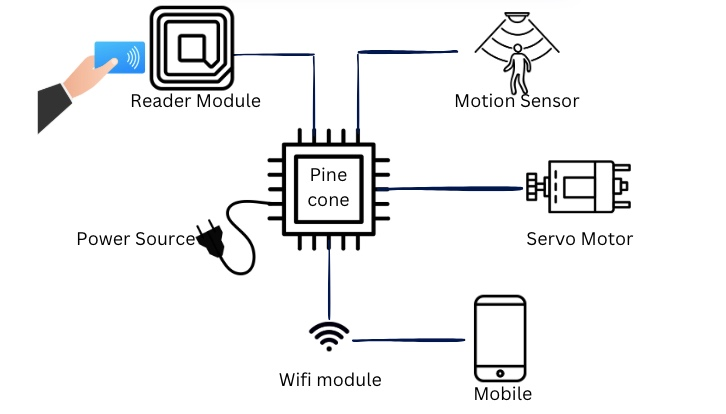
\includegraphics[width=0.5\textwidth]{architecture.jpeg}
    \caption{System Architecture of the SMART SECURITY DOOR LOCK SYSTEM with Servo Motor}
    \label{fig:system_architecture}
\end{figure}
	
	
	\section{Conclusion}
\label{sec:Conclusion}

Bringing our Smart Security Door Lock System to life has been a journey full of learning and adjustments. At first, we imagined a system packed with advanced features that would combine security, convenience, and modern technology. We wanted it to be more than just a door lock  it had to be a smarter, easier way to control access, stop unauthorized entry, and improve security for homes or offices.While building the system, we faced some challenges. Some parts didn’t work as expected, and it was difficult to put all our ideas together into one smooth design. To solve these issues, we simplified our approach and focused on making the system efficient and practical. Using the Pinecone microcontroller as the core, along with key components like the RFID reader, motion sensor, Wi-Fi module, and mobile app, we created a system that works effectively.

Although we couldn’t include every idea we started with, what we’ve built is strong, reliable, and highly functional. Our Smart Security Door Lock System isn’t just a lock it’s a complete solution designed to make security easier and more convenient. It uses motion sensors to detect activity, an RFID reader for secure access, and a mobile app that acts as a control panel for users. This makes managing security simple while keeping homes and offices safe.The idea of a smart security system combines  hardware, effective control features, and user friendly mobile app. Our system is an innovative step forward in IoT technology. It not only achieves the goals we set but also goes beyond our expectations in terms of usefulness and flexibility. By replacing traditional locks with modern technology, the Smart Security Door Lock System offers valuable benefits and a glimpse into the future of smart home security.Our system is ready to improve lives by offering a perfect mix of safety, convenience, and innovation.


	% Show cited references
	\printbibliography[title={References}]
\end{document}
